\documentclass[11pt]{article}
\usepackage[utf8]{inputenc}
\usepackage[T1]{fontenc}

\usepackage{bm}
\usepackage{amsmath}
\usepackage{siunitx}
\usepackage{graphicx}
\usepackage{xcolor}
\usepackage{fancyhdr}
\usepackage{wrapfig}
\usepackage{float}
\usepackage{enumitem}
\usepackage{multirow}
\usepackage{tikz}
\usepackage{titlesec}
\usepackage[small]{caption}

\usepackage[notes,backend=biber]{biblatex-chicago}
\usepackage[english]{babel}
\usepackage{csquotes}
\usepackage{hyperref}

\usepackage[margin=1in]{geometry}
\usepackage{setspace}
%\usepackage{newtxtext,newtxmath}

\pagestyle{fancy}
\fancyhf{}
\fancyhead[L]{JYZ314}
\fancyhead[R]{\thepage}
\renewcommand{\headrulewidth}{0pt}

\setlength{\headheight}{15.0pt}
\setlength{\parindent}{0pt}
\setlength{\parskip}{0.6em}

\titleformat*{\section}{\Large\bfseries}
\titleformat*{\subsection}{\large\bfseries}
\titlespacing*{\section}{0pt}{4pt}{4pt}
\titlespacing*{\subsection}{0pt}{4pt}{4pt}

\onehalfspacing

\captionsetup[figure]{font=small,justification=centering}

\bibliography{references}

% this expresses a regualar vector
\newcommand{\bvec}[1]{\bm{\mathbf{#1}}}

\begin{document}

	\begin{center}
		\textbf{\Large Investigating the relationship between the electric current and magnetic force exerted on a wire}

		\vspace*{8pt}

		May 2022
	\end{center}

    \section*{Introduction}

	\section*{Background}

\subsection*{Electromagnetism}

\begin{wrapfigure}[11]{r}{0.3\textwidth}
	\centering
	\vspace{-10pt}
	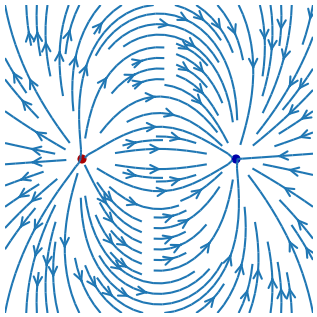
\includegraphics[width=0.3\textwidth]{figures/electric_field.png}
	\caption{Electric field around two opposing charges.}
	\label{fig:electric-field}
\end{wrapfigure}

Electromagnetism can ultimately thought of as the interaction between positively and negatively charged particles.
Charged particles are attracted to other particles of the opposite charge, and repelled by like charge.
Force exerted between two oppositely charged particles effects a region of space where other charges will be affected.
This is called an electric field and can be seen in Figure \ref{fig:electric-field} as depicted with field lines, where the arrows indicate the direction of the force experienced by a positive test charge.
The magnitude of the electric field at some point in space, as experienced by a positive test charge, is called the electric field strength, denoted $\bvec{E}$.
Generally, the field strength of an electric field is greater when it is closer to a charge.\footcite{britelectric}

\newpage

\begin{wrapfigure}[11]{r}{0.3\textwidth}
	\centering
	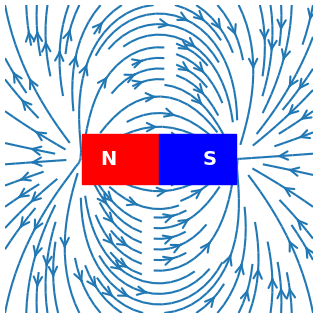
\includegraphics[width=0.3\textwidth]{figures/magnet_field.png}
	\caption{Magnetic field around a magnetic dipole.}
	\label{fig:magnet-field}
\end{wrapfigure}

In terms of magnetism, magnets embody this principle by having two poles, north and south, which could be thought of as positive and negative poles respectively.
In this way, opposite poles attract while like poles repel.
The region in which a magnetic dipole is effected by these forces is called a magnetic field and is depicted in Figure \ref{fig:magnet-field}.
The field lines of a magnetic field point from north to south.
There are two nearly identical vector fields that represent a magnetic field; magnetic field strength, $\bvec{H}$ or H-field, and magnetic flux density, $\bvec{B}$ or B-field.
While their differences are beyond the scope of this investigation, it is important to know that an H-field is concerned with the field strength of a specific point while a B-field is concerned with the density of the field lines at a specific point, also known as flux density.
This investigation concerns the latter field, magnetic flux density, and will refer to it as a magnetic field.\footcite{britfields}

Electricity also embodies this principle in electric current, where negatively charged electrons flow towards a more positive charge.
However, conventional thinking would have the direction of current as the movement from higher to lower charge, hence current flows from positive to negative.
This movement of charge is what creates magnetic fields.
Specifically, if current is moving through a wire, than the movement of charge creates a magnetic field whose field lines are concentric circles around the wire, perpendicular to the direction of current.\footcite{msufields}
Similar to how magnets can attract or repel each other, these moving charges are also subject to magnetic force.
This force, combined with electric force, is called Lorentz force.

\subsection*{Lorentz Force}

\begin{wrapfigure}[10]{r}{0.3\textwidth}
	\centering
	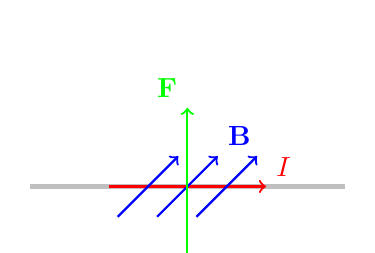
\begin{tikzpicture}
		\draw[ultra thick,lightgray] (-2,0,0) -- (2,0,0);
		\draw[thick,red,->] (-1,0,0) -- (1,0,0) node[above right]{$I$};
		\draw[thick,blue,->] (-0.5,0,1) -- (-0.5,0,-1);
		\draw[thick,blue,->] (0,0,1) -- (0,0,-1) node[above right]{$\bvec{B}$};
		\draw[thick,blue,->] (0.5,0,1) -- (0.5,0,-1);
		\draw[thick,green,->] (0,-1,0) -- (0,1,0) node[above left]{$\bvec{F}$};
	\end{tikzpicture}
	\caption{Force on a current-carrying wire. All vectors are perpendicular to each other.}
	\label{fig:laplace-force}
\end{wrapfigure}

Lorentz force, in terms of vectors, is defined as:
\begin{equation*}
	\bvec{F} = q\bvec{E} + q\bvec{v} \times \bvec{B}
\end{equation*}
where $q$ is the charge of a point particle, $\bvec{v}$ is the velocity of the particle, $\bvec{E}$ is the electric field, and $\bvec{B}$ is the magnetic field.
This equation represents the forces experienced by a charged particle in an electromagnetic field.
The cross product of $\bvec{v}$ and $\bvec{B}$ indicates that the force is perpendicular to both the direction of velocity and the magnetic field.\footcite{navelorentz}

\newpage

Lorentz force can be extended to describe the relationship between magnetic force and a current-carrying wire.
If the wire is placed in a uniform magnetic field with no electric field, then the equation simplifies to:
\begin{equation*}
	\bvec{F} = q\bvec{v} \times \bvec{B} \text{.}
\end{equation*}
Knowing that $\bvec{v}$ is the length of the wire $\bvec{L}$ divided by time $t$, and that current $I$ is the number of charged particles going through a point over time, the equation can then be rewritten to:\footcite{navelaplace}
\begin{align*}
	\bvec{F} &= q\frac{\bvec{L}}{t} \times \bvec{B} \\
	\bvec{F} &= \frac{q}{t}\bvec{L} \times \bvec{B} \\
	\bvec{F} &= I\bvec{L} \times \bvec{B} \text{.}
\end{align*}
This force is illustrated in Figure \ref{fig:laplace-force}, where current, B-field, and force are all perpendicular to each other.
Assuming that the current, B-field, and force are perpendicular to begin with, then the equation can be written as:
\begin{equation}
	F = ILB \label{eqn:laplace}
\end{equation}

\subsection*{Experimental Equation}

In order to test this relationship, one of the elements of Lorentz force must be used as the independent and dependent variables.
For the dependent variable, force is the most flexible variable to measure.
As for the independent variable, there are three options.
Looking at Equation \eqref{eqn:laplace}, of current, length, and B-field strength, current is the easiest to vary.
For B-field strength, either the type of magnet would be varied at the same distance from the wire, or the distance would be varied, of which the latter will be much more difficult since a magnetic field does not completely adhere to the inverse square law.\footcite{wwdistance}
As for length, a magnet would be required whose surface area could cover the range test lengths.
Current, on the other hand, can easily be varied by varying the voltage output of a power supply.
However, current should be limited to under two amps to reduce the chance of burns, whether it be electrical or heat emitted by components.
This means that force will inherently be quite small, even if its magnitude is scaled by using strong magnets.

In order to measure a small force, a pendulum apparatus similar to the CGI video demonstration by the National High Magnetic Field Laboratory will be used.\footcite{nmllorentz}
In theory, the pendulum will deflect to a specific angle in which gravity balances exerted Lorentz force.
Therefore, the deflection angle can be used to determine the Lorentz force through vector analysis.
Letting $\theta$ represent the deflection angle, $F$ represent the Lorentz force, and $T$ the tension on the pendulum wire, the relationship between gravity and $F$ is defined through the horizontal and vertical components of total force:
\begin{figure}[t!]
	\centering
	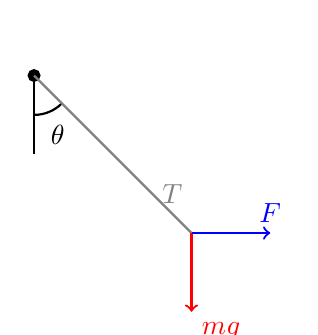
\begin{tikzpicture}
		\filldraw[ultra thick,black] (0,3) circle (1.5pt);
		\draw[thick] (0,2.5) arc [start angle=-90,end angle=-45,x radius=0.5,y radius=0.5];
		\node at (0.3,2.25) {$\theta$};
		\draw[thick,black] (0,3) -- (0,2); 
		\draw[thick,gray] (0,3) -- (2,1) node[near end,right]{$T$};
		\draw[thick,red,->] (2,1) -- (2,0) node[below right]{$mg$};
		\draw[thick,blue,->] (2,1) -- (3,1) node[above]{$F$};
	\end{tikzpicture}
	\caption{Vector diagram of total forces acting on the experiment apparatus.}
	\vspace{-1.5em}
	\label{fig:vector}
\end{figure}
\begin{align*}
	x:& \qquad -T \cos\theta + F =0 \\
	y:& \qquad T \sin\theta - mg =0
\end{align*}
Solving these equations by isolating and substituting T for one of the equations give the following:
\begin{equation}
	F = mg \tan\theta \text{.} \label{eqn:experiment}
\end{equation}
Thus, $F$ is proportional to $\tan\theta$. Expanding $F$ for $ILB$ and assuming $L$ and $B$ are constant, then $I$ is also proportional to $\tan\theta$.


	\section*{Experiment Design}

\subsection*{Hypothesis}

As the current going through the wire increase, the force acting on the wire due to a magnetic field will linearly increase. Hence, the deflection angle of the pendulum in the experiment will also increase.

\subsection*{Variables}

\textbf{Independent variable} --- current flowing through the wire of the pendulum, achieved through varying output voltage from the power supply.
Due to the inconsistent resistance of the circuit, caused by changing contact of the wire with the supports as it swings, exact current values cannot be achieved.
The target current values were $0.20\si{\ampere}$, $0.40\si{\ampere}$, $0.60\si{\ampere}$, $0.80\si{\ampere}$, $1.00\si{\ampere}$, $1.20\si{\ampere}$, and $1.40\si{\ampere}$.
These variables were measured with an uncertainty of $\pm0.01$ based off the readings from the power supply.

\textbf{Dependent variable} --- angle of deflection of the pendulum. The angle was measured through by imaging the deflecting pendulum at a flat plane and constant distance, then using a measurement tool from GIMP, an image processing software. The measurement uncertainty was $\pm0.01$.

\textbf{Controlled variables} --- the mass of the wire; $4.9\pm0.1\si{\gram}$ --- length of the copper wire under the magnetic field; $4.61\pm0.05\si{\centi\meter}$ --- vertical wire length; $5.56\pm0.05\si{\centi\meter}$ --- distance between magnets; $3.12\pm0.05\si{\centi\meter}$.
The wire is kept perpendicular to the magnetic field lines between the magnets.

\subsection*{Procedure}

\begin{enumerate}
	\item Gather a breadboard, two straightened, conductive, identical paper clips, needle nose pliers, and a spool of exposed copper wire to create the pendulum.
	\begin{enumerate}
		\item Using needle nose pliers, take the end of a straightened paper clip and bend it into a hinge that will act as a pivot for the pendulum wire.
		Create a hinge on the other paper clip such that the length of both paper clips are the same.
		Ensure the hinges overhang so that there is enough clearance between the hinges and the wire when it is placed.
		Place both paper clips at least $4\si{\centi\meter}$ away from each other on the breadboard; they will act as supports for the wire.
		\item Spool out an appropriate length of copper wire so that there is at least $5\si{\centi\meter}$ of length between the pivot and the lowest point of the wire.
		At least $15\si{\centi\meter}$ of wire should be used, with excess being used to secure the wire to the supports. 
		Using needle nose pliers, bend the ends of the wire into a U shape hook to allow the wire to hang from the supports.
		Bend the remaining wire into a square U shape such that the vertical segments are of equal length and the horizontal segment is roughly equal to the distance between the supports.
		\item Fit the wire into the supports and check if it can swing freely.
		If the wire does not swing freely, either minutely unbend the hinges on the supports or widen the U shape hooks at the end of the wire.
	\end{enumerate}
	\begin{figure}[H]
		\centering
		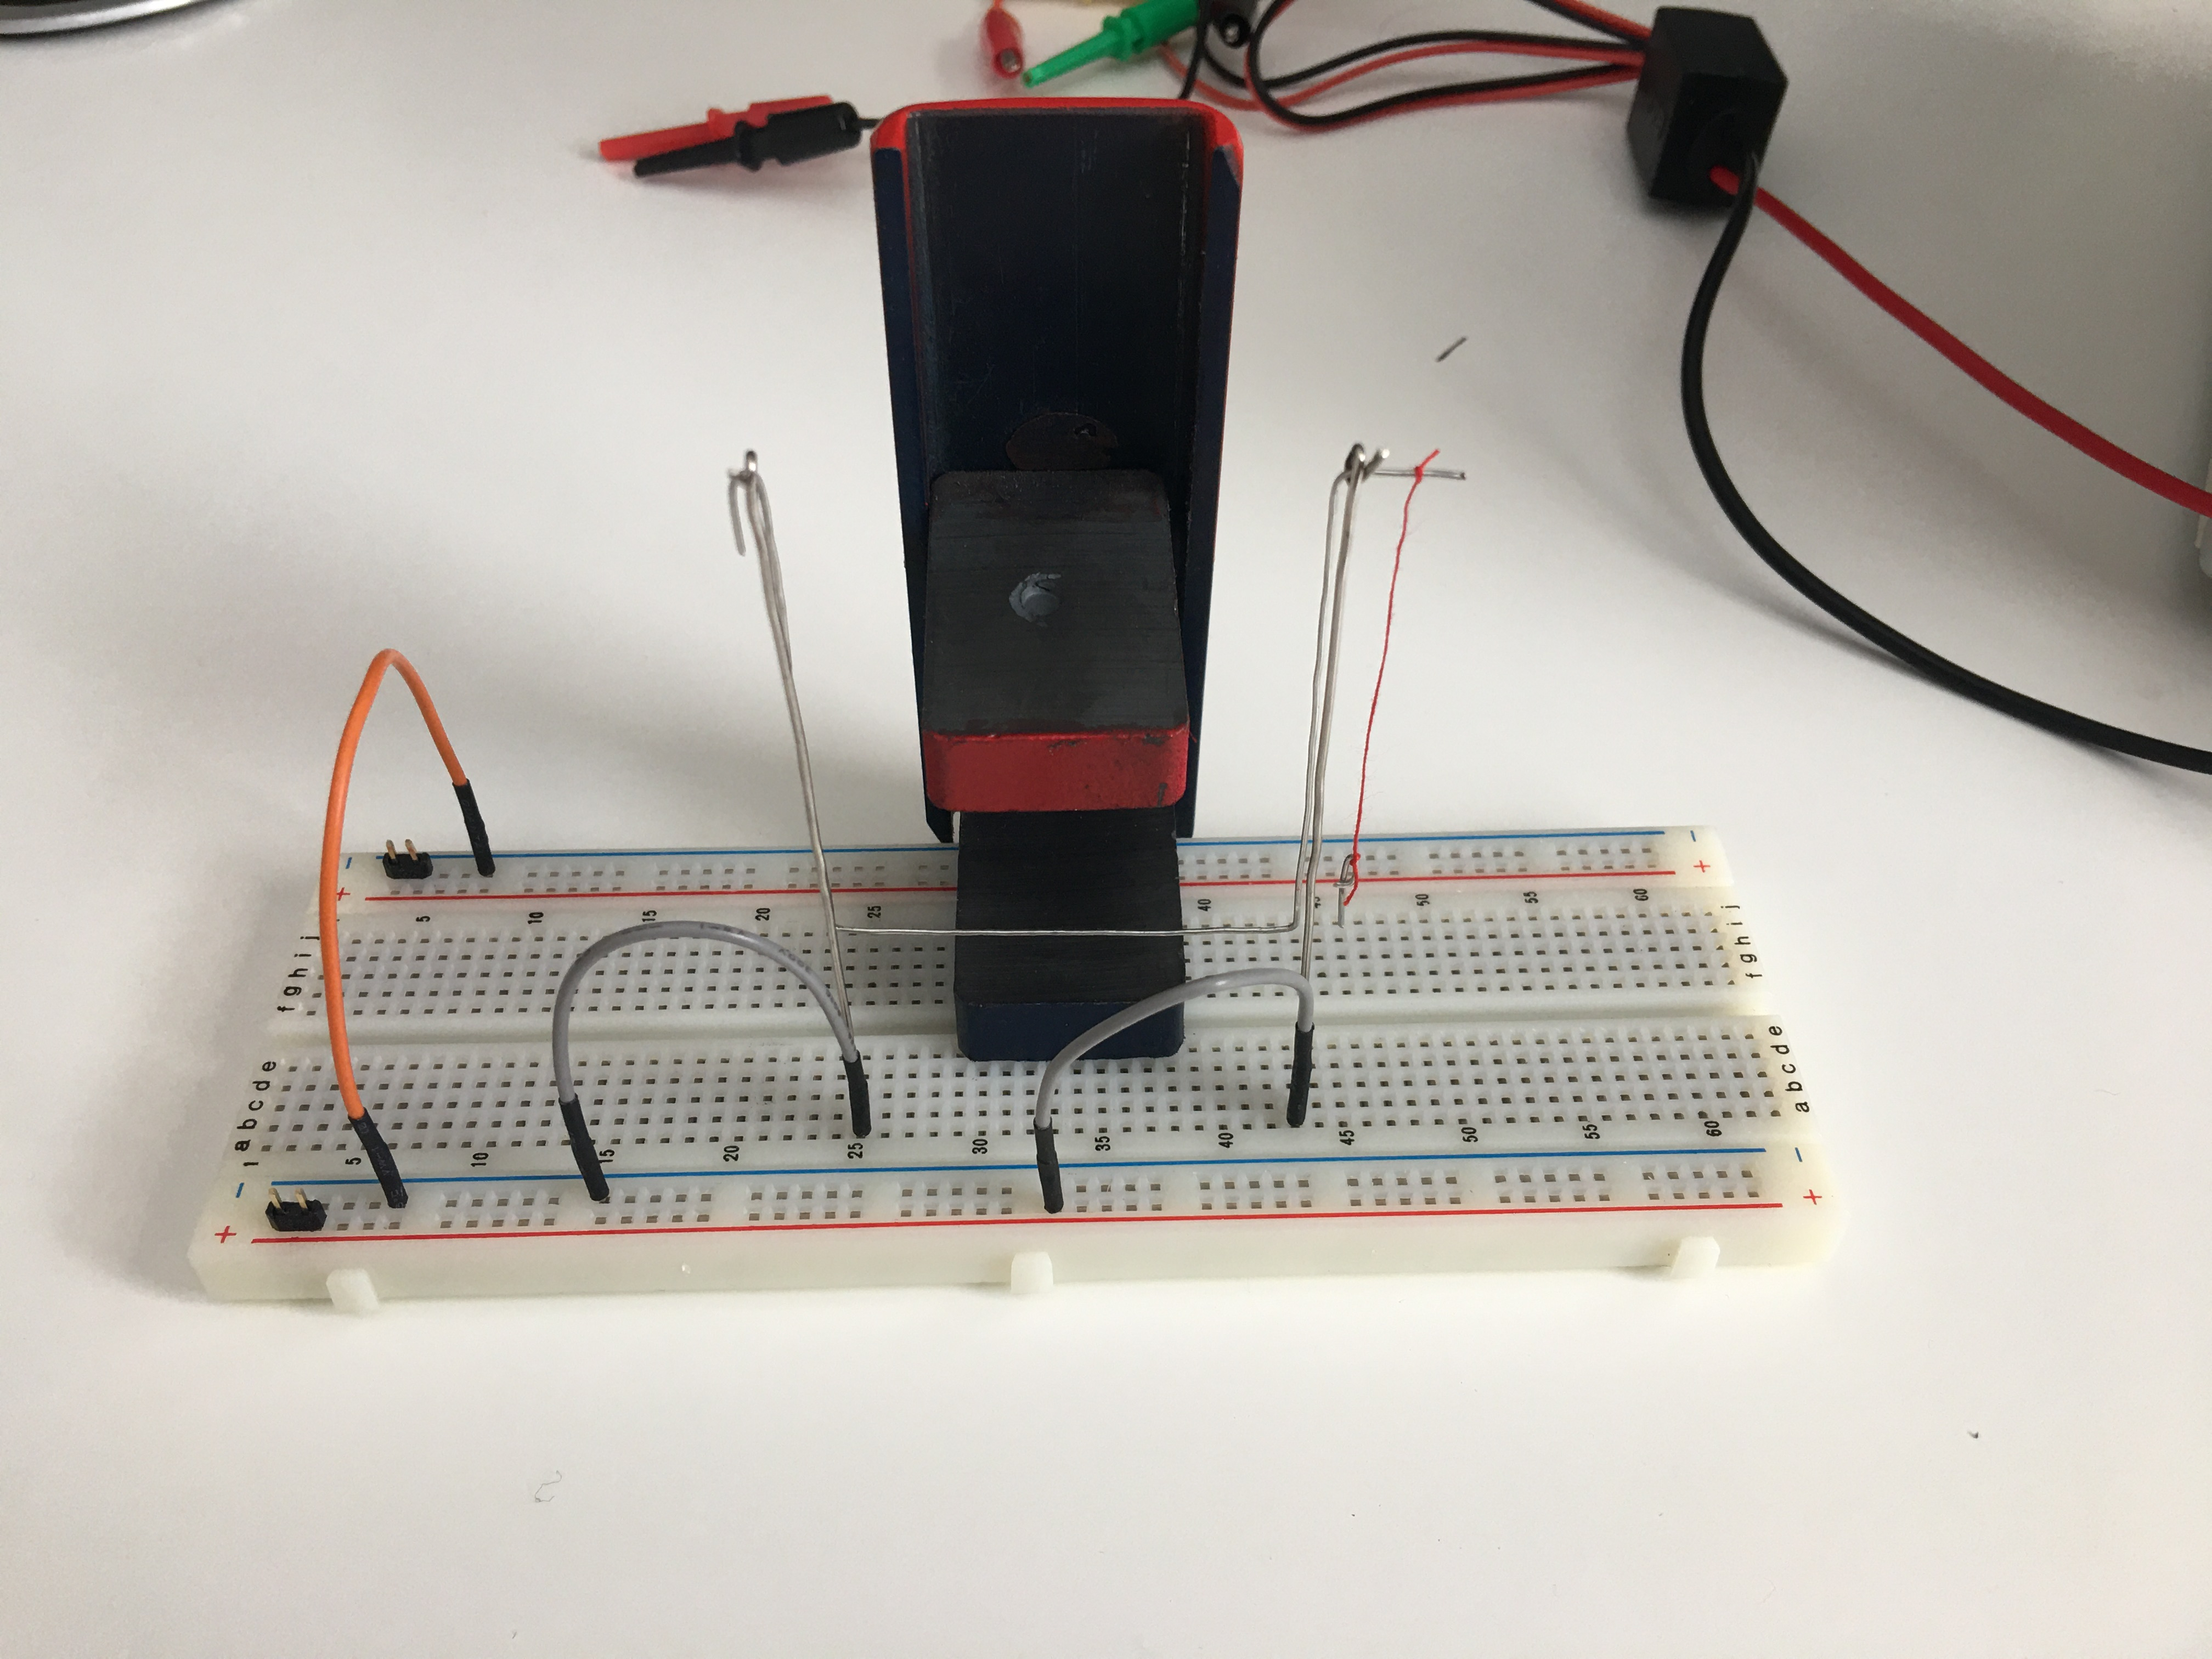
\includegraphics[width=0.5\textwidth]{figures/IMG_5514.JPG}
		\caption{Image of the experiment setup. The positive side of the wire is indicated by the red thread.}
		\label{fig:apparatus}
	\end{figure}
	\item Gather two large flat surface area magnets whose poles are on the largest face and a metal bracket which the magnets will be mounted onto.
	The magnets must have a large enough surface area to account for the expected deflection angle range.
	\begin{enumerate}
		\item Take note of the poles of each magnet.
		Identify which face of each magnet is north and south.
		\item Mount one magnet onto the bottom of the metal bracket with its south pole facing up.
		Mount the other magnet so that its south pole is also facing up, with the minimum amount of distance between the two magnets so that a uniform magnetic field is created, but does not result in the two magnets breaking off the mount and attracting each other.
		Also ensure that the distance between the two magnets is enough to account for the movement of the wire as its deflection angle increases.
		\item Place the mount onto the breadboard and in front of the wire.
		The wire should be within but on the edge of the magnetic field between the two magnets.
	\end{enumerate}
	\item Gather the power supply and necessary cables to provide current to the experiment.
	\begin{enumerate}
		\item Use jumper wires to connect the lanes of the supports to the power rails on the breadboard.
		When viewing the experiment perpendicular to the wire, make sure the pendulum is connect to the power rails so that conventional current flows from right to left.
		\item Verify that there are no potential short circuits on the breadboard.
		\item Connect the power supply to the power rails and provide $0.5\si{\volt}$ to the breadboard to test the setup.
		If everything is set up correctly, the wire should have deflected from the normal and away from the supports, into the magnets.
		If the wire deflects into the supports, switch around the direction of current in the pendulum setup.
		If the wire does not move, either the circuit is open somewhere, the hinges or hooks are too small, the wire is not making contact with the supports due to insulation, or the paperclips are not conductive.
		Troubleshoot each potential issue.
	\end{enumerate}
	\item Prop a camera or imaging sensor at least $15\si{\centi\meter}$ away from the apparatus and facing parallel to the length of the wire.
	Make sure the position and orientation of the camera to the apparatus remains the same throughout the experiment.
	The vertical segment of the wire should be on a single perpendicular plane relative to the camera and at the center of the image.
	\item Use the camera to photograph the deflection angle of the wire while at rest. \label{step:measure0}
	\item Provide enough voltage to the breadboard such that there is about $0.20\si{\ampere}$ going through the wire.
	Because the current may fluctuate as the wire swings, it is fine to around be within $\pm0.10\si{\ampere}$, so long as the current is no longer fluctuating and the wire is in a static equilibrium. \label{step:measure}
	\vspace{-1em} % something wrong went on here
	\begin{enumerate}
		\item If the power supply does not measure current, use a digital multimeter and connect one end to a support and the other to its respective power rail.
		\item Use the camera to photograph the deflection angle of the wire. 
	\end{enumerate}
	\item Repeat step \ref{step:measure} with $0.40\si{\ampere}$, $0.60\si{\ampere}$, $0.80\si{\ampere}$, $1.00\si{\ampere}$, $1.20\si{\ampere}$, and $1.40\si{\ampere}$.\label{step:repeat}
	\item Repeat steps \ref{step:measure0}, \ref{step:measure}, and \ref{step:repeat} four more times, ending with five trials.
\end{enumerate}

\subsection*{Safety Considerations}

As mentioned before, the current should be kept below $2.00\si{\ampere}$ to reduce the chance of a burn.
Parts of the apparatus may become hot, mainly the point of connection between the wire and the supports, so avoid touching those areas.
Keep the overall power output of the power supply below $4.00\si{\watt}$ so that there is not enough power to induce current through your body.
When handling strong magnets, avoid placing any bodily extremities between them, as they can potentially cause injury.


	\section*{Results}

\subsection*{Qualitative Observations}

The current going through the wire fluctuated as the wire swung, likely due to the changing contact of the wire with the supports.
There were specific ranges where the current would fluctuate, mainly at the lower currents.
At around $1.40\si{\ampere}$, the wire would get close enough to the bracket that it would jump and stick to the bracket.
This was mitigated by avoiding current from exceeding $1.50\si{\ampere}$.
From visual observation, the angle of deflection would increase as the current increased, but their relationship was determinable
from visuals.

\subsection*{Raw Data}

The data provided below shows the measured current and respective measured angle from 5 trials.
The angle measurements were done through the measurement tool in GIMP.

\begin{table}[H]
	\centering
	\setstretch{1.15}
	\begin{tabular}{|lr||lr||lr||lr||lr|}
		\hline
		\multicolumn{2}{|c||}{Trial 1} & \multicolumn{2}{|c||}{Trial 2} & \multicolumn{2}{c||}{Trial 3}& \multicolumn{2}{c||}{Trial 4}& \multicolumn{2}{c|}{Trial 5} \\
		\hline
		$I(\si{\ampere})$ & $\theta(\si{\degree})$ & $I(\si{\ampere})$ & $\theta(\si{\degree})$ & $I(\si{\ampere})$ & $\theta(\si{\degree})$ & $I(\si{\ampere})$ & $\theta(\si{\degree})$ & $I(\si{\ampere})$ & $\theta(\si{\degree})$ \\
		$\pm0.01$ & $\pm0.01$ & $\pm0.01$ & $\pm0.01$ & $\pm0.01$ & $\pm0.01$ & $\pm0.01$ & $\pm0.01$ & $\pm0.01$ & $\pm0.01$ \\
		\hline
		0 & 0.62 & 0 & 0.48 & 0 & 0.57 & 0 & 0.57 & 0 & 0.66 \\
		0.22 & 5.53 & 0.23 & 6.83 & 0.26 & 6.62 & 0.18 & 4.11 & 0.19 & 4.37 \\
		0.39 & 12.02 & 0.42 & 12.63 & 0.46 & 13.65 & 0.39 & 11.3 & 0.44 & 13.25 \\
		0.58 & 17.41 & 0.59 & 17.78 & 0.57 & 16.88 & 0.61 & 17.82 & 0.61 & 18.14 \\
		0.80 & 22.02 & 0.88 & 23.49 & 0.78 & 21.65 & 0.83 & 22.64 & 0.82 & 22.35 \\
		1.04 & 25.84 & 1.01 & 25.51 & 1.01 & 25.47 & 1.06 & 25.98 & 0.99 & 25.05 \\
		1.20 & 28.59 & 1.21 & 27.82 & 1.20 & 28.29 & 1.22 & 28.44 & 1.18 & 27.78 \\
		1.42 & 31.65 & 1.40 & 30.84 & 1.41 & 31.23 & 1.42 & 30.93 & 1.38 & 30.41 \\
		\hline
	\end{tabular}
	\caption{Raw data table of measured angles $\theta$ for increasing values of $I$ over 5 trials.}
	\label{tab:raw1}
\end{table}

\newpage

\subsection*{Processed Data}

To account for a potential offset in angle due to the shape of the wire, the measured angle of the wire at rest is subtracted from all other measurements.
This was calculated as:
\begin{equation*}
	\theta_{\text{final}} = \theta_{\text{measured}} - \theta_0 \text{.}
\end{equation*}
For example, the for the first data point, $5.53\si{\degree} - 0.62\si{\degree} = 4.91\si{\degree}$.
The uncertainty of the measured angle was propagated as such:
\begin{equation*}
	\Delta\theta_{\text{final}} = \Delta\theta_{\text{measured}} + \Delta\theta_0 \text{.}
\end{equation*}
For the first data point, $\pm(0.01 + 0.01)\si{\degree} = \pm0.02\si{\degree}$.
This was done for each trial.

The average deflection angle for each target current (ie. $0.20\si{\ampere}$, $0.40\si{\ampere}$, etc.) will not be taken, given the inherent variation of current. % I am going to regret this.

\begin{table}[H]
	\centering
	\setstretch{1.15}
	\begin{tabular}{|lr||lr||lr||lr||lr|}
		\hline
		\multicolumn{2}{|c||}{Trial 1} & \multicolumn{2}{|c||}{Trial 2} & \multicolumn{2}{c||}{Trial 3}& \multicolumn{2}{c||}{Trial 4}& \multicolumn{2}{c|}{Trial 5} \\
		\hline
		$I(\si{\ampere})$ & $\theta(\si{\degree})$ & $I(\si{\ampere})$ & $\theta(\si{\degree})$ & $I(\si{\ampere})$ & $\theta(\si{\degree})$ & $I(\si{\ampere})$ & $\theta(\si{\degree})$ & $I(\si{\ampere})$ & $\theta(\si{\degree})$ \\
		$\pm0.01$ & $\pm0.02$ & $\pm0.01$ & $\pm0.02$ & $\pm0.01$ & $\pm0.02$ & $\pm0.01$ & $\pm0.02$ & $\pm0.01$ & $\pm0.02$ \\
		\hline
		0.22 & 4.91 & 0.23 & 6.35 & 0.26 & 6.05 & 0.18 & 3.54 & 0.19 & 3.71 \\
		0.39 & 11.40 & 0.42 & 12.15 & 0.46 & 13.08 & 0.39 & 10.73 & 0.44 & 12.59 \\
		0.58 & 16.79 & 0.59 & 17.30 & 0.57 & 16.31 & 0.61 & 17.25 & 0.61 & 17.48 \\
		0.80 & 21.40 & 0.88 & 23.01 & 0.78 & 21.08 & 0.83 & 22.07 & 0.82 & 21.69 \\
		1.04 & 25.22 & 1.01 & 25.03 & 1.01 & 24.90 & 1.06 & 25.41 & 0.99 & 24.39 \\
		1.20 & 27.97 & 1.21 & 27.34 & 1.20 & 27.72 & 1.22 & 27.87 & 1.18 & 27.12 \\
		1.42 & 31.03 & 1.40 & 30.36 & 1.41 & 30.66 & 1.42 & 30.36 & 1.38 & 29.75 \\
		\hline
	\end{tabular}
	\caption{Corrected angle data table for measured angles $\theta$.}
	\vspace{-10pt}
	\label{tab:raw2}
\end{table}

The data in Table \ref{tab:raw2} is plotted in Figure \ref{fig:rawplot}.

Next, the corrected angle data was used to calculate the force exerted on the wire by using Equation \eqref{eqn:experiment}, where $m = 4.9\pm0.1\si{\gram}$ and $g = 9.81\si{\meter\per\second\squared}$. The first data point was calculated as:
\begin{equation*}
	4.9\si{\gram} \times 9.81\si{\meter\per\second\squared} \times \tan 4.91\si{\degree} = 4.13\si{\milli\newton} \text{.}
\end{equation*}
Propagation of uncertainty was calculated as:
\begin{equation*}
	\Delta F = \left( \frac{1}{\tan\theta} \times \frac{\tan(\theta + \Delta\theta) - \tan(\theta - \Delta\theta)}{2} + \frac{\Delta m}{m} \right) \times F \text{.}
\end{equation*}
For the first data point, the uncertainty for the $\tan\theta$ calculation was determined to be:
\begin{equation*}
	\frac{\tan([4.91 + 0.02]\si{\degree}) - \tan([4.91 - 0.02]\si{\degree})}{2} = 3.52\times10^{-4} \text{.}
\end{equation*}
Then, the sum of the fractional uncertainties between $\tan\theta$ and mass were taken:
\begin{equation*}
	\frac{3.52\times10^{-4}}{\tan 4.91\si{\degree}} + \frac{0.1\si{\gram}}{4.9\si{\gram}} = 2.5\times10^{-2} \text{.}
\end{equation*}
Finally, the fractional uncertainty is converted to the absolute uncertainty of the final value of force:
\begin{equation*}
	2.5\times10^{-2} \times 4.13\si{\milli\newton} = \pm 0.10\si{\milli\newton}
\end{equation*}
The data from these calculations are displayed on Table \ref{tab:proc} and plotted in Figure \ref{fig:procplot}.

\begin{figure}[t!]
	\centering
	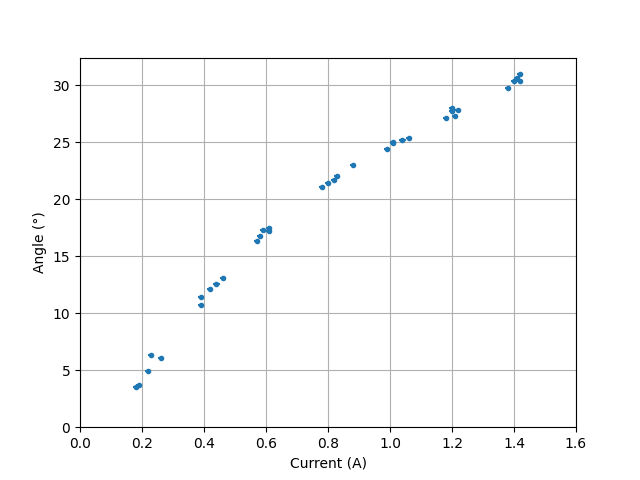
\includegraphics[width=0.75\textwidth]{figures/rawplot.png}
	\caption{Graph of corrected measured angles vs. current. Note that the errorbars are so small that they are barely visible in the graph.}
	\label{fig:rawplot}
\end{figure}

\begin{table}[H]
	\centering
	\setstretch{1.15}
	\begin{tabular}{|ccc||ccc||ccc|}
		\hline
		\multicolumn{3}{|c||}{Trial 1} & \multicolumn{3}{c||}{Trial 2} & \multicolumn{3}{c|}{Trial 3} \\
		\hline
		$I(\si{\ampere})$ & $F(\si{\milli\newton})$ & $\Delta F(\si{\milli\newton})$ & $I(\si{\ampere})$ & $F(\si{\milli\newton})$ & $\Delta F(\si{\milli\newton})$ & $I(\si{\ampere})$ & $F(\si{\milli\newton})$ & $\Delta F(\si{\milli\newton})$ \\
		$\pm0.01$ & & & $\pm0.01$ & & & $\pm0.01$ & & \\
		\hline
		0.22 & 4.13 & $\pm0.10$ & 0.23 & 5.35 & $\pm0.13$ & 0.26 & 5.09 & $\pm0.12$ \\
		0.39 & 9.69 & $\pm0.22$ & 0.42 & 10.35 & $\pm0.23$ & 0.46 & 11.17 & $\pm0.25$ \\
		0.58 & 14.50 & $\pm0.31$ & 0.59 & 14.97 & $\pm0.32$ & 0.57 & 14.07 & $\pm0.31$ \\
		0.80 & 18.84 & $\pm0.40$ & 0.88 & 20.41 & $\pm0.44$ & 0.78 & 18.53 & $\pm0.40$ \\
		1.04 & 22.64 & $\pm0.48$ & 1.01 & 22.45 & $\pm0.48$ & 1.01 & 22.31 & $\pm0.48$ \\
		1.20 & 25.53 & $\pm0.54$ & 1.21 & 24.85 & $\pm0.53$ & 1.20 & 25.26 & $\pm0.54$ \\
		1.42 & 28.92 & $\pm0.61$ & 1.40 & 28.16 & $\pm0.60$ & 1.41 & 28.50 & $\pm0.60$\\
		\hline
	\end{tabular}
	\begin{tabular}{|ccc||ccc|}
		\hline
		\multicolumn{3}{|c||}{Trial 4} & \multicolumn{3}{c|}{Trial 5} \\
		\hline
		$I(\si{\ampere})$ & $F(\si{\milli\newton})$ & $\Delta F(\si{\milli\newton})$ & $I(\si{\ampere})$ & $F(\si{\milli\newton})$ & $\Delta F(\si{\milli\newton})$ \\
		$\pm0.01$ & & & $\pm0.01$ & & \\
		\hline
		0.18 & 2.97 & $\pm0.08$ & 0.19 & 3.12 & $\pm0.08$ \\
		0.39 & 9.11 & $\pm0.20$ & 0.44 & 10.74 & $\pm0.24$ \\
		0.61 & 14.93 & $\pm0.32$ & 0.61 & 15.14 & $\pm0.33$ \\
		0.83 & 19.49 & $\pm0.42$ & 0.82 & 19.12 & $\pm0.41$ \\
		1.06 & 22.84 & $\pm0.49$ & 0.99 & 21.79 & $\pm0.47$ \\
		1.22 & 25.42 & $\pm0.54$ & 1.18 & 24.62 & $\pm0.52$ \\
		1.42 & 28.16 & $\pm0.60$ & 1.38 & 27.47 & $\pm0.58$ \\
		\hline
	\end{tabular}
	\caption{Table of force in relation to current.}
	\vspace{-10pt}
	\label{tab:proc}
\end{table}

\begin{figure}[b!]
	\centering
	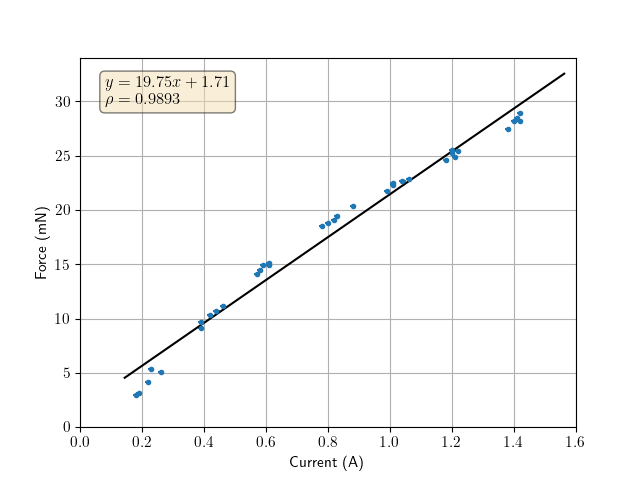
\includegraphics[width=0.75\textwidth]{figures/procplot.png}
	\caption{Graph of force vs. time.}
	\label{fig:procplot}
\end{figure}


	\section*{Discussion}

While the points on Figure \ref{fig:procplot} are visibly correlated and have a strong correlation coefficient with the plotted regression, the shape of the points suggests the current induced in the wire and the force measured are closely but not linearly related.
Given that the random error is too small to result in meaningful differences, this means that either there exists systematic error in the experiment, the hypothesis that current is linearly related to force is incorrect, 

There are a few possibilities that could have led to the deviation from the hypothesis.
Friction between the supports and the wire can explain the qualitative observation of fluctuation between currents.
In addition to the changing points of contact resulting in varying current as the pendulum swings, friction between the hooks of the wire and the hinges of the supports would create resistance torque which would set a force threshold before the wire can deflect.
While this does explain the fluctuations in current and erratic swinging, the resistance torque should not increase as the deflection angle increases.
This is because, as the deflection angle increases, the weight of the wire will become distributed between the supports and the end of the vertical length of the wire (the bottom of the wire), of which will be supported by the Lorentz force.
In addition, friction was considered in the procedure, where the hinges had to be loose enough to allow the wire to swing freely.
Given an analysis of torque on the experiment is beyond the scope of this investigation, the best guess that can be given is that friction is insignificant to the results of the experiment.

Another possibility is the experiment failed to consider the force of attraction between the supports and the wire.
Since both are conductors and have current flowing between them, they will create a magnetic field that will influence the other, hence experience attraction or repulsion between each other.
Knowing from Lorentz force, if current in one wire is going the opposite direction of current in the other wire, they will repel each other, which could attribute to a slight increase in force at lower deflection angles.
The force exerted between the two wires can be estimated by using the definition of the ampere:
``One ampere is defined as the current that would cause a force of $2 \times 10^{-7}\si{\newton}$ per metre between two long parallel conductors separated by $1\si{\meter}$ in a vacuum.''\footcite{pearsonamp}
Right away, $2 \times 10^{-7}\si{\newton}$ is three orders of magnitude below the measured force, meaning that, even with one ampere going through the wire, the contributing force would be unnoticeable.
This means the attraction between the supports and the wire is not the main cause of the deviation from a linear relation in the experiment.

Since, the horizontal segment of the wire did vary in distance between the magnets, it is possible that the B-field varied by a significant amount as the wire swung during the experiment.
Although magnetic field strength does not exactly follow the inverse square law, its strength still decreases substantially with distance.
At the minimum and maximum deflection angles (around $5\si{\degree}$ or $30\si{\degree}$) the magnetic field could have been stronger than the rest of the angles.
However, the opposite is reflected in the data in Figure \ref{fig:procplot}, as force at the low and high currents are below the linear regression, while points in the middle are above the linear regression.
This does not mean variation in magnetic field strength is ruled out.
There is the possibility that, despite using large magnets, the magnetic field between the two magnets was not uniform.
Using the magnetic gap calculator from K{\&}J Magnetics, the magnetic field strength relative to the distance from the center axis between two cylindrical magnets can be determined.\footcite{kjgap}
By approximating the dimensions of the experiment magnets as cylindrical magnets and setting an arbitrary magnetic strength (similar to the magnets used in the experiment), the graph in Figure \ref{fig:gaps} was produced.
\begin{figure}[H]
	\centering
	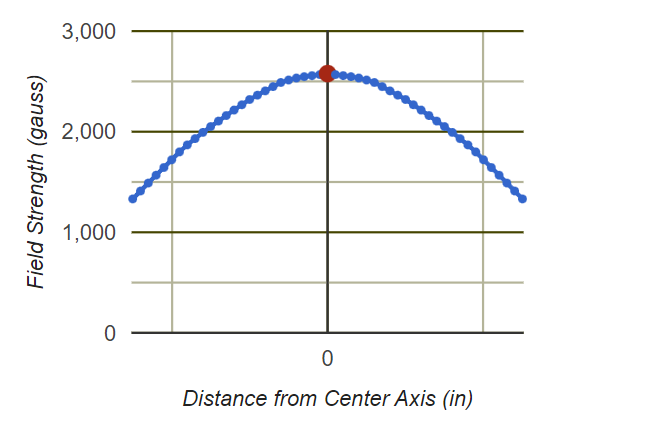
\includegraphics[width=0.5\textwidth]{figures/gapplot.PNG}
	\caption{Distribution of field strength over distance from the center axis between two magnets.}
	\label{fig:gaps}
	\vspace{-1em}
\end{figure}
This would explain why the force at the minimum and maximum angles varies from a linear relation; the magnetic field strength decreases when the wire is further away from the center.
While the geometry between rectangular and cylindrical magnets are different, it is likely this concept is still present in rectangular magnets.
Therefore, the variation of the data from a linear relation is due to the non-uniformity of the magnetic field between the two magnets.

\section*{Evaluation}

Because the magnetic field used in the experiment was not uniform, thus leading to the non-linear relation, it is difficult to determine if the data supports the hypothesis.
While it is possible to correct the data based on the field strength profile of the magnets used, all that is known is that they are ferrite magnets; their grades are unknown.
This means their field strength profile cannot be determined.


	\section*{Conclusion}

With regards to the hypothesis that current is linearly proportional to the magnetic force exerted on a wire, the methods and experiment used ultimately resulted in data that partially supports the hypothesis.
Having not considered that the strength of the magnetic field varies with position, there exists systematic error which makes it difficult to judge whether the relation between the current and force is linear.
In addition, the design of the experiment had created some complications with measurement and resulted in minor skewing of the data.
Nevertheless, from Figure \ref{fig:procplot}, it is clear that they are correlated such that they are proportional.
This evidence is consistent with Lorentz force, which describes the connection between electric charge and magnetism.

\section*{Improvements for Future Investigation}

As suggested in the evaluation, conducting the experiment at a larger scale would make angle measurements easier, potentially reduce current fluctuations, and resolve the issue of the wire's proximity to the magnets.
Using copper tape and a copper pipe will further reduce current fluctuations and issues regarding friction.
Stronger magnets with larger surface area, preferably neodymium bar magnets with the poles on the long edge, as well as utilizing larger currents can allow for a wider range of deflection angles.
And finally, to prevent the same mistakes of this investigation, the magnet composition and grade---specifically its magnetic flux density---should be known, and variation of field strength around the two magnets at a specific separation distance should be measured prior to beginning the trials.

	\newpage

	\printbibliography[
		heading=bibintoc,
		title={Bibliography}
	]
	
	\vfill
	
	%All elements of this IA are available on GitHub: \url{https://github.com/fellow-sh/PhysicsIA}

\end{document}
